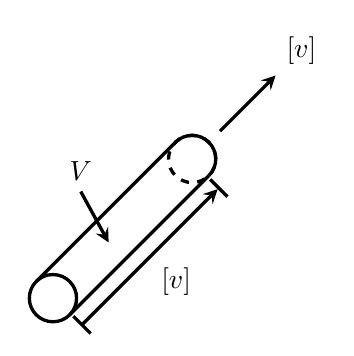
\begin{tikzpicture}[line width = 1.2pt, line join=round,x={(-0.35355cm,-0.35355cm)},y={(1cm, 0cm)},z={(0cm,1cm)},>=stealth]
	% Querschnittsflächen
	\draw [dashed] (0,0) circle (0.3cm);
	\draw (0,0,0)++(0,{0.3*sqrt(2)/2},{-0.3*sqrt(2)/2}) arc (-45:135:0.3cm);
	\draw (5,0) circle (0.3cm);
	% Begrenzungen
	\coordinate (a) at (5,0,0);
	\coordinate (ah) at (2.5,{0.5*sqrt(2)/2},{-0.5*sqrt(2)/2});
	\draw (0,{0.3*sqrt(2)/2},{-0.3*sqrt(2)/2}) -- ++(a);
	\draw (0,{-0.3*sqrt(2)/2},{0.3*sqrt(2)/2}) -- ++(a);
	% differentielles Wegstück
	\draw [|<-|] (0,{0.5*sqrt(2)/2},{-0.5*sqrt(2)/2}) -- ++(a);
	\draw (ah) node[anchor=north west] {$\upd \weg[v]$};
	% Geschwindigkeit
	\draw [->] (-1,0,0) -- (-3,0,0) node[anchor=south west] {$\geschw[v]$};
	% ladungsdichte
	\draw [<-] (3,0,0) -- (4,0,1) node[anchor=south] {$\laddichte{V}$};
\end{tikzpicture}